% Options for packages loaded elsewhere
\PassOptionsToPackage{unicode}{hyperref}
\PassOptionsToPackage{hyphens}{url}
\PassOptionsToPackage{dvipsnames,svgnames*,x11names*}{xcolor}
%
\documentclass[
  12pt,
  brazilian,
]{book}
\usepackage{amsmath,amssymb}
\usepackage{lmodern}
\usepackage{ifxetex,ifluatex}
\ifnum 0\ifxetex 1\fi\ifluatex 1\fi=0 % if pdftex
  \usepackage[T1]{fontenc}
  \usepackage[utf8]{inputenc}
  \usepackage{textcomp} % provide euro and other symbols
\else % if luatex or xetex
  \usepackage{unicode-math}
  \defaultfontfeatures{Scale=MatchLowercase}
  \defaultfontfeatures[\rmfamily]{Ligatures=TeX,Scale=1}
\fi
% Use upquote if available, for straight quotes in verbatim environments
\IfFileExists{upquote.sty}{\usepackage{upquote}}{}
\IfFileExists{microtype.sty}{% use microtype if available
  \usepackage[]{microtype}
  \UseMicrotypeSet[protrusion]{basicmath} % disable protrusion for tt fonts
}{}
\makeatletter
\@ifundefined{KOMAClassName}{% if non-KOMA class
  \IfFileExists{parskip.sty}{%
    \usepackage{parskip}
  }{% else
    \setlength{\parindent}{0pt}
    \setlength{\parskip}{6pt plus 2pt minus 1pt}}
}{% if KOMA class
  \KOMAoptions{parskip=half}}
\makeatother
\usepackage{xcolor}
\IfFileExists{xurl.sty}{\usepackage{xurl}}{} % add URL line breaks if available
\IfFileExists{bookmark.sty}{\usepackage{bookmark}}{\usepackage{hyperref}}
\hypersetup{
  pdftitle={R na Cozinha},
  pdfauthor={Paulo Guilherme Pinheiro dos Santos},
  pdflang={pt-br},
  colorlinks=true,
  linkcolor=red,
  filecolor=Maroon,
  citecolor=blue,
  urlcolor=magenta,
  pdfcreator={LaTeX via pandoc}}
\urlstyle{same} % disable monospaced font for URLs
\usepackage[top=3cm,left=3cm,right=2cm,bottom=2cm]{geometry}
\usepackage{color}
\usepackage{fancyvrb}
\newcommand{\VerbBar}{|}
\newcommand{\VERB}{\Verb[commandchars=\\\{\}]}
\DefineVerbatimEnvironment{Highlighting}{Verbatim}{commandchars=\\\{\}}
% Add ',fontsize=\small' for more characters per line
\usepackage{framed}
\definecolor{shadecolor}{RGB}{248,248,248}
\newenvironment{Shaded}{\begin{snugshade}}{\end{snugshade}}
\newcommand{\AlertTok}[1]{\textcolor[rgb]{0.94,0.16,0.16}{#1}}
\newcommand{\AnnotationTok}[1]{\textcolor[rgb]{0.56,0.35,0.01}{\textbf{\textit{#1}}}}
\newcommand{\AttributeTok}[1]{\textcolor[rgb]{0.77,0.63,0.00}{#1}}
\newcommand{\BaseNTok}[1]{\textcolor[rgb]{0.00,0.00,0.81}{#1}}
\newcommand{\BuiltInTok}[1]{#1}
\newcommand{\CharTok}[1]{\textcolor[rgb]{0.31,0.60,0.02}{#1}}
\newcommand{\CommentTok}[1]{\textcolor[rgb]{0.56,0.35,0.01}{\textit{#1}}}
\newcommand{\CommentVarTok}[1]{\textcolor[rgb]{0.56,0.35,0.01}{\textbf{\textit{#1}}}}
\newcommand{\ConstantTok}[1]{\textcolor[rgb]{0.00,0.00,0.00}{#1}}
\newcommand{\ControlFlowTok}[1]{\textcolor[rgb]{0.13,0.29,0.53}{\textbf{#1}}}
\newcommand{\DataTypeTok}[1]{\textcolor[rgb]{0.13,0.29,0.53}{#1}}
\newcommand{\DecValTok}[1]{\textcolor[rgb]{0.00,0.00,0.81}{#1}}
\newcommand{\DocumentationTok}[1]{\textcolor[rgb]{0.56,0.35,0.01}{\textbf{\textit{#1}}}}
\newcommand{\ErrorTok}[1]{\textcolor[rgb]{0.64,0.00,0.00}{\textbf{#1}}}
\newcommand{\ExtensionTok}[1]{#1}
\newcommand{\FloatTok}[1]{\textcolor[rgb]{0.00,0.00,0.81}{#1}}
\newcommand{\FunctionTok}[1]{\textcolor[rgb]{0.00,0.00,0.00}{#1}}
\newcommand{\ImportTok}[1]{#1}
\newcommand{\InformationTok}[1]{\textcolor[rgb]{0.56,0.35,0.01}{\textbf{\textit{#1}}}}
\newcommand{\KeywordTok}[1]{\textcolor[rgb]{0.13,0.29,0.53}{\textbf{#1}}}
\newcommand{\NormalTok}[1]{#1}
\newcommand{\OperatorTok}[1]{\textcolor[rgb]{0.81,0.36,0.00}{\textbf{#1}}}
\newcommand{\OtherTok}[1]{\textcolor[rgb]{0.56,0.35,0.01}{#1}}
\newcommand{\PreprocessorTok}[1]{\textcolor[rgb]{0.56,0.35,0.01}{\textit{#1}}}
\newcommand{\RegionMarkerTok}[1]{#1}
\newcommand{\SpecialCharTok}[1]{\textcolor[rgb]{0.00,0.00,0.00}{#1}}
\newcommand{\SpecialStringTok}[1]{\textcolor[rgb]{0.31,0.60,0.02}{#1}}
\newcommand{\StringTok}[1]{\textcolor[rgb]{0.31,0.60,0.02}{#1}}
\newcommand{\VariableTok}[1]{\textcolor[rgb]{0.00,0.00,0.00}{#1}}
\newcommand{\VerbatimStringTok}[1]{\textcolor[rgb]{0.31,0.60,0.02}{#1}}
\newcommand{\WarningTok}[1]{\textcolor[rgb]{0.56,0.35,0.01}{\textbf{\textit{#1}}}}
\usepackage{longtable,booktabs,array}
\usepackage{calc} % for calculating minipage widths
% Correct order of tables after \paragraph or \subparagraph
\usepackage{etoolbox}
\makeatletter
\patchcmd\longtable{\par}{\if@noskipsec\mbox{}\fi\par}{}{}
\makeatother
% Allow footnotes in longtable head/foot
\IfFileExists{footnotehyper.sty}{\usepackage{footnotehyper}}{\usepackage{footnote}}
\makesavenoteenv{longtable}
\usepackage{graphicx}
\makeatletter
\def\maxwidth{\ifdim\Gin@nat@width>\linewidth\linewidth\else\Gin@nat@width\fi}
\def\maxheight{\ifdim\Gin@nat@height>\textheight\textheight\else\Gin@nat@height\fi}
\makeatother
% Scale images if necessary, so that they will not overflow the page
% margins by default, and it is still possible to overwrite the defaults
% using explicit options in \includegraphics[width, height, ...]{}
\setkeys{Gin}{width=\maxwidth,height=\maxheight,keepaspectratio}
% Set default figure placement to htbp
\makeatletter
\def\fps@figure{htbp}
\makeatother
\setlength{\emergencystretch}{3em} % prevent overfull lines
\providecommand{\tightlist}{%
  \setlength{\itemsep}{0pt}\setlength{\parskip}{0pt}}
\setcounter{secnumdepth}{5}
\usepackage{booktabs}
\ifxetex
  % Load polyglossia as late as possible: uses bidi with RTL langages (e.g. Hebrew, Arabic)
  \usepackage{polyglossia}
  \setmainlanguage[variant=brazilian]{portuguese}
\else
  \usepackage[main=brazilian]{babel}
% get rid of language-specific shorthands (see #6817):
\let\LanguageShortHands\languageshorthands
\def\languageshorthands#1{}
\fi
\ifluatex
  \usepackage{selnolig}  % disable illegal ligatures
\fi
\usepackage[]{natbib}
\bibliographystyle{apalike}

\title{R na Cozinha}
\author{Paulo Guilherme Pinheiro dos Santos}
\date{30 de junho de 2021}

\begin{document}
\maketitle

{
\hypersetup{linkcolor=}
\setcounter{tocdepth}{1}
\tableofcontents
}
\hypertarget{apresentauxe7uxe3o}{%
\chapter{Apresentação}\label{apresentauxe7uxe3o}}

Neste guia, pretendemos compartilhar nossa experiência no uso do \emph{software} \texttt{R} com a comunidade com o objetivo de contribuir com tudo que o programa nos ofereceu ao longo desses anos de uso.

\ldots{}

\hypertarget{intro}{%
\chapter{Introdução}\label{intro}}

\begin{Shaded}
\begin{Highlighting}[]
\FunctionTok{par}\NormalTok{(}\AttributeTok{mar =} \FunctionTok{c}\NormalTok{(}\DecValTok{4}\NormalTok{, }\DecValTok{4}\NormalTok{, .}\DecValTok{1}\NormalTok{, .}\DecValTok{1}\NormalTok{))}
\FunctionTok{plot}\NormalTok{(pressure, }\AttributeTok{type =} \StringTok{\textquotesingle{}b\textquotesingle{}}\NormalTok{, }\AttributeTok{pch =} \DecValTok{19}\NormalTok{)}
\end{Highlighting}
\end{Shaded}

\begin{figure}

{\centering 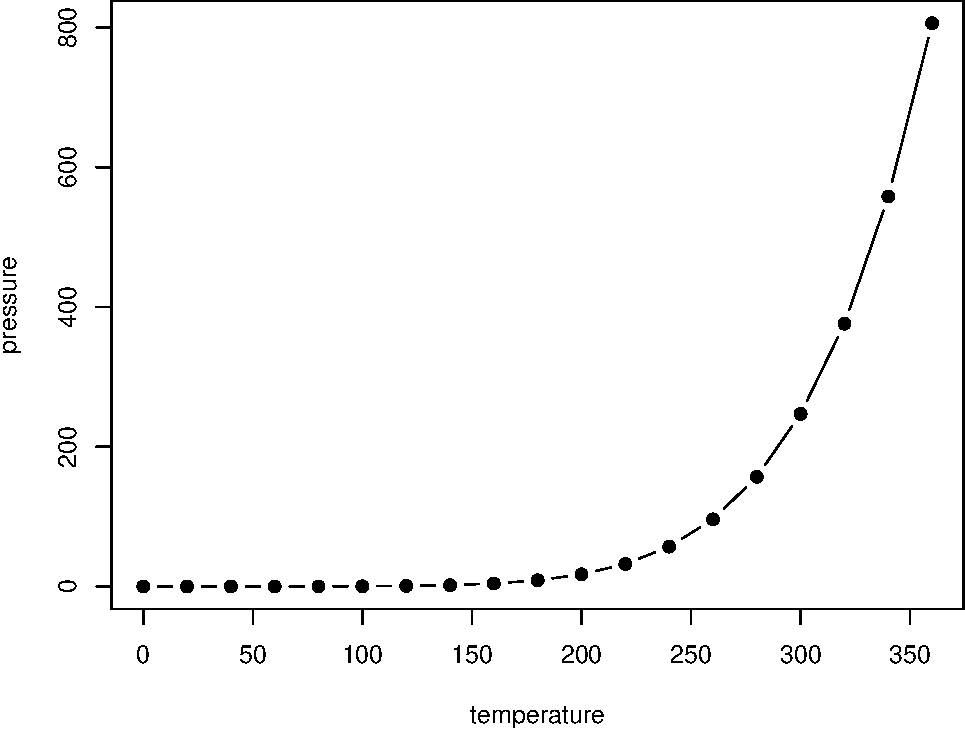
\includegraphics[width=0.8\linewidth]{R_pg2_book_files/figure-latex/nice-fig-1} 

}

\caption{Here is a nice figure!}\label{fig:nice-fig}
\end{figure}

\begin{Shaded}
\begin{Highlighting}[]
\NormalTok{knitr}\SpecialCharTok{::}\FunctionTok{kable}\NormalTok{(}
  \FunctionTok{head}\NormalTok{(iris, }\DecValTok{20}\NormalTok{), }\AttributeTok{caption =} \StringTok{\textquotesingle{}Here is a nice table!\textquotesingle{}}\NormalTok{,}
  \AttributeTok{booktabs =} \ConstantTok{TRUE}
\NormalTok{)}
\end{Highlighting}
\end{Shaded}

\begin{table}

\caption{\label{tab:nice-tab}Here is a nice table!}
\centering
\begin{tabular}[t]{rrrrl}
\toprule
Sepal.Length & Sepal.Width & Petal.Length & Petal.Width & Species\\
\midrule
5.1 & 3.5 & 1.4 & 0.2 & setosa\\
4.9 & 3.0 & 1.4 & 0.2 & setosa\\
4.7 & 3.2 & 1.3 & 0.2 & setosa\\
4.6 & 3.1 & 1.5 & 0.2 & setosa\\
5.0 & 3.6 & 1.4 & 0.2 & setosa\\
\addlinespace
5.4 & 3.9 & 1.7 & 0.4 & setosa\\
4.6 & 3.4 & 1.4 & 0.3 & setosa\\
5.0 & 3.4 & 1.5 & 0.2 & setosa\\
4.4 & 2.9 & 1.4 & 0.2 & setosa\\
4.9 & 3.1 & 1.5 & 0.1 & setosa\\
\addlinespace
5.4 & 3.7 & 1.5 & 0.2 & setosa\\
4.8 & 3.4 & 1.6 & 0.2 & setosa\\
4.8 & 3.0 & 1.4 & 0.1 & setosa\\
4.3 & 3.0 & 1.1 & 0.1 & setosa\\
5.8 & 4.0 & 1.2 & 0.2 & setosa\\
\addlinespace
5.7 & 4.4 & 1.5 & 0.4 & setosa\\
5.4 & 3.9 & 1.3 & 0.4 & setosa\\
5.1 & 3.5 & 1.4 & 0.3 & setosa\\
5.7 & 3.8 & 1.7 & 0.3 & setosa\\
5.1 & 3.8 & 1.5 & 0.3 & setosa\\
\bottomrule
\end{tabular}
\end{table}

\hypertarget{matemuxe1tica-buxe1sica-no-r}{%
\chapter{\texorpdfstring{Matemática básica no \texttt{R}}{Matemática básica no R}}\label{matemuxe1tica-buxe1sica-no-r}}

Aqui mostramos como executar algumas operações aritméticas básicas e algumas funções no \texttt{R}. Trazemos os códigos e ao final um vídeo explicativo com todas as operações listadas.

\hypertarget{aritmuxe9tica}{%
\section{Aritmética}\label{aritmuxe9tica}}

\begin{Shaded}
\begin{Highlighting}[]
\CommentTok{\# Soma:}
\DecValTok{1}\SpecialCharTok{+}\DecValTok{3}
\DecValTok{10}\SpecialCharTok{+}\DecValTok{2}

\CommentTok{\# Subtração:}
\DecValTok{5{-}2}
\DecValTok{10{-}2}
\DecValTok{2{-}10}

\CommentTok{\# Multiplicação;}
\DecValTok{2}\SpecialCharTok{*}\DecValTok{3}
\DecValTok{7}\SpecialCharTok{*}\DecValTok{4}

\CommentTok{\# Potenciação}
\DecValTok{2}\SpecialCharTok{\^{}}\DecValTok{3}
\DecValTok{4}\SpecialCharTok{\^{}}\DecValTok{4}
\DecValTok{2}\SpecialCharTok{**}\DecValTok{3}
\DecValTok{4}\SpecialCharTok{**}\DecValTok{4}

\CommentTok{\# Divisão;}
\DecValTok{8}\SpecialCharTok{/}\DecValTok{2}
\DecValTok{10}\SpecialCharTok{/}\DecValTok{3}

\CommentTok{\# Quociente da divisão; parte inteira: \%/\%}
\DecValTok{10}\SpecialCharTok{\%/\%}\DecValTok{3}

\CommentTok{\# Resto da divisão: \%\%}
\DecValTok{10}\SpecialCharTok{\%\%}\DecValTok{3}

\CommentTok{\# Módulo:}
\FunctionTok{abs}\NormalTok{(}\SpecialCharTok{{-}}\DecValTok{3}\NormalTok{)}
\FunctionTok{abs}\NormalTok{(}\DecValTok{8}\NormalTok{)}
\FunctionTok{abs}\NormalTok{(}\SpecialCharTok{{-}}\DecValTok{10}\NormalTok{)}

\CommentTok{\# Logarítmo:}
\FunctionTok{log}\NormalTok{(}\DecValTok{2}\NormalTok{)}
\FunctionTok{log}\NormalTok{(}\DecValTok{2}\NormalTok{,}\DecValTok{10}\NormalTok{)}
\FunctionTok{log10}\NormalTok{(}\DecValTok{2}\NormalTok{)}
\NormalTok{?log}
\FunctionTok{help}\NormalTok{(log)}
\FunctionTok{log}\NormalTok{(}\DecValTok{2}\NormalTok{,}\FunctionTok{exp}\NormalTok{(}\DecValTok{1}\NormalTok{))}
\NormalTok{log}

\CommentTok{\# Exponencial:}
\FunctionTok{exp}\NormalTok{(}\DecValTok{1}\NormalTok{)}
\FunctionTok{exp}\NormalTok{(}\DecValTok{3}\NormalTok{)}
\FunctionTok{exp}\NormalTok{(}\DecValTok{0}\NormalTok{)}

\CommentTok{\# Pi}
\NormalTok{pi}

\CommentTok{\# Funções Trigonométricas:}
\NormalTok{?sin}
\FunctionTok{sin}\NormalTok{(pi}\SpecialCharTok{/}\DecValTok{2}\NormalTok{)}
\FunctionTok{sinpi}\NormalTok{(}\DecValTok{1}\SpecialCharTok{/}\DecValTok{2}\NormalTok{)}
\FunctionTok{cos}\NormalTok{(pi}\SpecialCharTok{/}\DecValTok{2}\NormalTok{)}
\FunctionTok{cos}\NormalTok{(pi)}
\FunctionTok{cos}\NormalTok{(}\DecValTok{0}\NormalTok{)}
\FunctionTok{tan}\NormalTok{(pi}\SpecialCharTok{/}\DecValTok{4}\NormalTok{)}
\FunctionTok{sin}\NormalTok{(pi}\SpecialCharTok{/}\DecValTok{4}\NormalTok{)}\SpecialCharTok{/}\FunctionTok{cos}\NormalTok{(pi}\SpecialCharTok{/}\DecValTok{4}\NormalTok{)}

\CommentTok{\# Fatorial:}
\FunctionTok{factorial}\NormalTok{(}\DecValTok{4}\NormalTok{)}
\DecValTok{4}\SpecialCharTok{*}\DecValTok{3}\SpecialCharTok{*}\DecValTok{2}\SpecialCharTok{*}\DecValTok{1}

\CommentTok{\# Combinações:}
\FunctionTok{choose}\NormalTok{(}\DecValTok{10}\NormalTok{,}\DecValTok{2}\NormalTok{)}
\DecValTok{10}\SpecialCharTok{*}\DecValTok{9}\SpecialCharTok{/}\FunctionTok{factorial}\NormalTok{(}\DecValTok{2}\NormalTok{)}
\FunctionTok{factorial}\NormalTok{(}\DecValTok{10}\NormalTok{)}\SpecialCharTok{/}\NormalTok{(}\FunctionTok{factorial}\NormalTok{(}\DecValTok{10{-}2}\NormalTok{)}\SpecialCharTok{*}\FunctionTok{factorial}\NormalTok{(}\DecValTok{2}\NormalTok{))}

\CommentTok{\# Somatórios:}
\NormalTok{x }\OtherTok{=} \DecValTok{3}\SpecialCharTok{:}\DecValTok{13}
\NormalTok{x}
\FunctionTok{sum}\NormalTok{(x)}
\FunctionTok{cumsum}\NormalTok{(x)}
\FunctionTok{max}\NormalTok{(}\FunctionTok{cumsum}\NormalTok{(x))}
\NormalTok{x }\SpecialCharTok{|}\ErrorTok{\textgreater{}} \FunctionTok{cumsum}\NormalTok{() }\SpecialCharTok{|}\ErrorTok{\textgreater{}} \FunctionTok{max}\NormalTok{()}

\CommentTok{\# Produtórios:}
\NormalTok{x }\SpecialCharTok{|}\ErrorTok{\textgreater{}} \FunctionTok{prod}\NormalTok{()}
\FunctionTok{prod}\NormalTok{(x)}
\end{Highlighting}
\end{Shaded}

\begin{itemize}
\tightlist
\item
  \emph{Link} da aula: \href{https://youtu.be/QDLqS3y5u7Q}{Matemática Básica no R}.
\end{itemize}

\hypertarget{operador-pipe}{%
\section{\texorpdfstring{Operador \emph{Pipe}}{Operador Pipe}}\label{operador-pipe}}

Aqui temos um exemplo básico da utilização do operador \emph{pipe} \texttt{\textbar{}\textgreater{}}disponível no \texttt{R} a partir deste ano de 2021.`

\begin{itemize}
\tightlist
\item
  \emph{Link} da aula: \href{https://youtu.be/n27-lBxdfFg}{Operador Pipe}.
\end{itemize}

\hypertarget{como-carregar-dados-para-o-r}{%
\chapter{\texorpdfstring{Como carregar dados para o \texttt{R}}{Como carregar dados para o R}}\label{como-carregar-dados-para-o-r}}

Neste capítulo mostraremos como importar base de dados ao \texttt{R}. Apresentaremos tanto exemplos com arquivos localizados num repositório local em seu computador, quanto disponíveis na \emph{web}.

\hypertarget{exemplo-1-o-pacote-datasets}{%
\section{\texorpdfstring{Exemplo 1: o pacote \texttt{datasets}}{Exemplo 1: o pacote datasets}}\label{exemplo-1-o-pacote-datasets}}

\hypertarget{exemplo-2}{%
\section{Exemplo 2:}\label{exemplo-2}}

\hypertarget{exemplo-3-importauxe7uxe3o-das-bases-de-covid-19}{%
\section{Exemplo 3: importação das bases de covid-19}\label{exemplo-3-importauxe7uxe3o-das-bases-de-covid-19}}

\hypertarget{jhu}{%
\subsection{JHU}\label{jhu}}

\hypertarget{br-ms}{%
\subsection{BR-MS}\label{br-ms}}

\hypertarget{pacote-coronabr}{%
\subsection{\texorpdfstring{Pacote \texttt{coronabr}}{Pacote coronabr}}\label{pacote-coronabr}}

\hypertarget{visualizauxe7uxe3o-de-dados}{%
\chapter{Visualização de dados}\label{visualizauxe7uxe3o-de-dados}}

Neste capítulo apresentaremos como utilizar o pacote \texttt{ggplot2} para visualização de dados.

\hypertarget{a-gramuxe1tica-dos-gruxe1ficos}{%
\section{A gramática dos gráficos}\label{a-gramuxe1tica-dos-gruxe1ficos}}

Antes de abordarmos o pacote \texttt{ggplot2}, vamos conversar um pouco sobre a lógica na qual ele foi concebido.

Mas, o que é uma gramática?

No geral, consiste num conjunto de regras. Sob a ótica da linguística, consiste num sistema formal de regras para gerar definições válidas numa língua.

\hypertarget{distribuiuxe7uxf5es-de-probabilidade}{%
\chapter{Distribuições de Probabilidade}\label{distribuiuxe7uxf5es-de-probabilidade}}

\hypertarget{modelo-uniforme-discreto}{%
\section{Modelo Uniforme Discreto}\label{modelo-uniforme-discreto}}

\hypertarget{modelo-de-bernoulli}{%
\section{Modelo de Bernoulli}\label{modelo-de-bernoulli}}

\hypertarget{modelo-binomial}{%
\section{Modelo Binomial}\label{modelo-binomial}}

\hypertarget{modelo-de-poisson}{%
\section{Modelo de Poisson}\label{modelo-de-poisson}}

\hypertarget{modelo-geomuxe9trico}{%
\section{Modelo Geométrico}\label{modelo-geomuxe9trico}}

\hypertarget{modelo-hipergeomuxe9trico}{%
\section{Modelo Hipergeométrico}\label{modelo-hipergeomuxe9trico}}

\hypertarget{modelo-uniforme-contuxednuo}{%
\section{Modelo Uniforme Contínuo}\label{modelo-uniforme-contuxednuo}}

\hypertarget{modelo-exponencial}{%
\section{Modelo Exponencial}\label{modelo-exponencial}}

\hypertarget{modelo-normal}{%
\section{Modelo Normal}\label{modelo-normal}}

\hypertarget{modelo-gamma}{%
\section{Modelo Gamma}\label{modelo-gamma}}

\hypertarget{modelo-beta}{%
\section{Modelo Beta}\label{modelo-beta}}

\hypertarget{modelo-qui-quadrado}{%
\section{Modelo Qui-quadrado}\label{modelo-qui-quadrado}}

\hypertarget{modelo-t-student}{%
\section{\texorpdfstring{Modelo \emph{t-Student}}{Modelo t-Student}}\label{modelo-t-student}}

\hypertarget{modelo-f-snedecor}{%
\section{\texorpdfstring{Modelo \emph{F-Snedecor}}{Modelo F-Snedecor}}\label{modelo-f-snedecor}}

\hypertarget{controle-de-fluxo}{%
\chapter{Controle de fluxo}\label{controle-de-fluxo}}

\hypertarget{ifcond-expr}{%
\section{if(cond) expr}\label{ifcond-expr}}

\hypertarget{ifcond-cons.expr-else-alt.expr}{%
\section{if(cond) cons.expr else alt.expr}\label{ifcond-cons.expr-else-alt.expr}}

\hypertarget{forvar-in-seq-expr}{%
\section{for(var in seq) expr}\label{forvar-in-seq-expr}}

\hypertarget{whilecond-expr}{%
\section{while(cond) expr}\label{whilecond-expr}}

\hypertarget{repeat-expr}{%
\section{repeat expr}\label{repeat-expr}}

\hypertarget{break}{%
\section{break}\label{break}}

\hypertarget{next}{%
\section{next}\label{next}}

\hypertarget{r-rstudio-git-github}{%
\chapter{\texorpdfstring{\(R + RStudio + Git + GitHub\)}{R + RStudio + Git + GitHub}}\label{r-rstudio-git-github}}

Neste capítulo vamos aprender como integrar o \texttt{R} e o \texttt{RStudio} ao \texttt{GitHub} utilizando o sistema de versionamento \texttt{Git}.

\hypertarget{como-fazer-com-r}{%
\chapter{\texorpdfstring{Como fazer 📚 com \texttt{R}}{Como fazer 📚 com R}}\label{como-fazer-com-r}}

\begin{Shaded}
\begin{Highlighting}[]
\NormalTok{emo}\SpecialCharTok{::}\FunctionTok{ji}\NormalTok{(}\StringTok{\textquotesingle{}poop\textquotesingle{}}\NormalTok{)}
\end{Highlighting}
\end{Shaded}

\begin{verbatim}
## 💩
\end{verbatim}

\hypertarget{como-fazer-blogs-com-r}{%
\chapter{\texorpdfstring{Como fazer \emph{blogs} com \texttt{R}}{Como fazer blogs com R}}\label{como-fazer-blogs-com-r}}

Aqui usaremos o pacote \texttt{blogdown} na criação e o \texttt{GitHub} para hospedagem.

\hypertarget{apresentauxe7uxf5es-com-r}{%
\chapter{\texorpdfstring{Apresentações com \texttt{R}}{Apresentações com R}}\label{apresentauxe7uxf5es-com-r}}

Com \texttt{R} podemos criar apresentações de diversas maneiras. Inclusive com o \texttt{RStudio} aumentamos mais ainda esse leque de possibilidades. Aqui mostraremos como fazê-las utilizando os pacotes \texttt{rmarkdown} e \texttt{xaringan}.

\hypertarget{considerauxe7uxf5es-finais}{%
\chapter{Considerações Finais}\label{considerauxe7uxf5es-finais}}

We have finished a nice book.

\renewcommand{\bibname}{Referências}
\addcontentsline{toc}{chapter}{Referências}

\hypertarget{appendix-apuxeandice}{%
\appendix}


\hypertarget{como-ter-mensagem-personalizada-ao-iniciar-o-r}{%
\chapter{\texorpdfstring{Como ter mensagem personalizada ao iniciar o \texttt{R}}{Como ter mensagem personalizada ao iniciar o R}}\label{como-ter-mensagem-personalizada-ao-iniciar-o-r}}

Aqui mostraremos como acessar e editar o arquivo \texttt{.Rprofile} para termos, por exemplo, uma mensagem personalizada ao iniciar uma sessão no \texttt{R}.

\href{https://stackoverflow.com/questions/46819684/how-to-access-and-edit-rprofile}{Link: clique aqui 🔗}

\hypertarget{section}{%
\chapter{}\label{section}}

  \bibliography{book.bib,packages.bib}

\end{document}
